\subsection{Implementation}\label{redundancy_implementation}

%	- You have to describe all that in your work, how do you define Main Partial/Full and Benefit Partial/Full, so how do you decide that. And generating this JSON_Report and filling this table is all interesting implementation information.
% Then comes the implementation what we implemented in the implementation and how did we test it?
% in the i\begin{center}


\end{center}mplementation then I go to specific implementation problems that I had with Henshin, maybe I didn't know how the rules were generated, how they did it, then you can show code snippets, and show a bit but not the whole code in the work
% the implementation and also the tests I run with the existing USs and see what comes out right.


\subsection{Test}\label{redundancy_test}

% here should explain what was the reiquirement and why
\begin{figure}[h]
\center
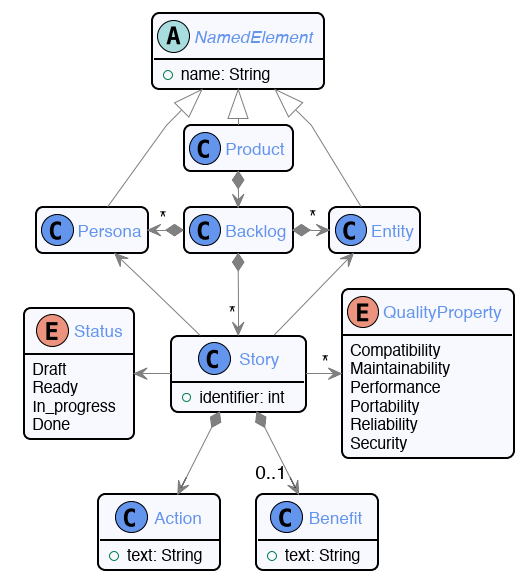
\includegraphics{Backlog_conceptual_metamodel}
\caption{Backlog conceptual metamodel \cite{mosser2022modelling}}\label{fig:conceptual_metamodel}


 
\subsection{Evaluation}\label{redundancy_evaluation}
%In this section we will present the results of applying our approach to analyse USs in 19 by CRF tool annotated backlog datasets. 
%The purpose of this section is to assess the effectiveness of our approach in analysing redundancy between USs. This section serves several key objective:
In this section, we address two different research questions and provide a detailed explanation of the experimental design and execution for each question. We also present a detailed analysis of the results to provide answers to these research questions, highlight their implications and provide insights into the research findings.
%\begin{itemize}
%	\item Demonstrating the validity and reliability of our proposed methodology for identifying and categorising redundancies between USs.
%	\item Presenting the results of our analysis across multiple datasets, highlighting the prevalence of \enquote{Full and Partial Redundancy} for both the main and benefit parts of USs.
%	\item Gaining insights into the nature and extent of redundancies between USs and its potential impact on software development processes.
%	\item Comparing results from different data sets, identifying patterns or trends and analysing variations in redundancy levels.
%\end{itemize}
\subsubsection*{Research Questions}
The research questions addressed in this section are as follows:
\begin{enumerate}
	\item Does our tool reliably determine the level of redundancy —either partial or full— between different parts of USs (main and benefit)?
	\item How does the tool's performance scale when the number of USs in a backlog increases?
	\end{enumerate}
\subsubsection*{Methodology}
To address the first questions "Does our tool reliably determine the level of redundancy—either partial or full—between different parts of USs (main and benefit)?", we recap the methodology employed to analyse redundancy between USs. We utilized a systematic approach that involved several key steps:
\begin{itemize}
	
	\item Data Collection: For a comprehensive assessment, we applied our approach to 19 backlog datasets presented by Mosser et al.\footnote{https://github.com/ace-design/nlp-stories}. They applied the Doccano approach to these publicly available requirements datasets\cite{requirementsdatasets}.
	
	It is also worth noting that some backlog datasets (g02, g13, g17, g27) did not follow the expected sentence structure, which is why we did not include them in the evaluation results to avoid unexpected behaviour. Table \ref{tb:backlogs} shows the project number of each dataset and the count of USs.
	%	- You have to describe all that in your work, how do you define Main Partial/Full and Benefit Partial/Full, so how do you decide that. And generating this JSON_Report and filling this table is all interesting implementation information.
	
	%When evaluating, I use tools on a large scale and I go through all the cases and look at what comes out of the use case as a meaningful result. As an evaluation, I will enter all the datasets we have as input and then what comes out will be 
	\begingroup
	\centering
	\scriptsize
	\renewcommand{\arraystretch}{1.5} 
	%\keepXColumns
	\begin{tabularx}{\linewidth}{l|XXXXXXXXXXXXXXXXXXX|X}
		Item&	1&	2&	3&	4&	5&	6&	7&	8&	9&	10&	11&	12&	13&	14&	15&	16&	17&	18&	19&	\\
		\hline
		%Project Name&loudoun&recycling&openspending&frictionless&scrumalliance	&nsf&camperplus&datahub&mis&neurohub&alfred&badcamp&rdadmp&archivesspace	&unibath&duraspace&racdam&culrepo&zooniverse&\\
		Project Nr.&	g03	&g04	&g05	&g08	&g10	&g11	&g12	&g14	&g16	&g18	&g19	&g21	&g22	&g23	&g24	&g25	&g26	&g27	&g28	&Total USs\\
		\hline
		Total USs&	57&	51	&53	&66	&97	&73	&54	&67	&66	&102	&137	&69	&83	&56	&53	&100	&100	&114	&60	&1458 \\
		\caption{Project number and count of USs contained in each backlog dataset}\label{tb:backlogs}
	\end{tabularx}	
	\endgroup
	
	%\item Preprocessing: Using the generated JSON report file for each dataset, we create a VBA script called \textit{extractFromJSONFiles}\footnote{https://github.com/amirrabieyannejad/USs\_Annotation/tree/main/Skript/extractFromJSONFiles} to iterate through all the JSON report files and extract the information such as \enquote{US-pair}, \enquote{US-text}, \enquote{total redundancy clauses}, \enquote{main redundancy clauses}, \enquote{benefit redundancy clauses} and \enquote{project number} and collect them all in an Excel file to perform further analyses.
	
	\item Identification of main and benefit parts: Each US was divided into its main part, which is the core functionality, and its benefit part, which describes the value to the persona.
	
	\item Detection of overlapping clauses: Recognition of overlapping clauses between a US-pair in a specific part of the USs.
	
	\item Redundancy analysis in main and benefit parts: Based on the redundant clauses identified, an automatic redundancy analysis was performed for the main and benefit parts of the US-pair based on certain criteria indicating the level of redundancy (partial or full) in the main and benefit parts.
		
	%\item Preprocessing: \item preprocessing: We transform each data set into graph transformation rules, apply CDA and generate a textual report in which each redundancy clause between US-pairs is marked with a hash symbol. Additionally,  the number of founded redundancies in the main and benefit sections is also determined.
\end{itemize}
\subsubsection*{Ground Truth Evaluation of US Redundancy}
Answering the first research question requires our automated system to have a reference point against which its accuracy can be measured. This reference point or "ground truth" is derived from a personal assessment and serves as a benchmark for the tool's performance.

In contrast to the tool evaluation, we did not evaluate based on labels (e.g., action, entity, persona, targets, etc.) in the personal evaluation. This means that when evaluating ground truth, we evaluate partial and full redundancy based on the phrases occurring in a given part as a one-to-one comparison.

The ground truth is the final assessment against which automated results are compared. It is derived from the personal judgement of a subject matter expert (in this case myself) using a combination of expertise, experience and specific evaluation criteria. The personal assessment is targeted at providing a reliable and accurate reference for redundancy between USs.\\\\
	The following criteria were taken into account in the personal assessment:
	\begin{itemize}
		\item A US-pair is evaluated as fully redundant in the main part, if all phrases occurred in the main parts of both USs fully overlap with one-to-one comparison. For example, the following US-pair is assessed as fully redundant:\\
		user\_story\_01: "\#g14\# as a \#publisher\#, i want to \#publish\# a \#dataset\#, so that i can view just the dataset with a few people."
		
		user\_story\_02: "\#g14\# as a \#publisher\#, i want to \#publish\# a \#dataset\#, so that i can share the dataset publicly with everyone."
		
		\item A US-pair is considered fully redundant in the main part, if all phrases in the main part of at least one US completely overlap. For instance:\\
		user\_story\_22: "\#g14\# as a \#consumer\#, i want to \#view\# a \#data package\# online, so that i can \#get\# a \#sense\# of whether this is the dataset i want."
		
		user\_story\_24: "\#g14\# as a \#consumer\#, i want to \#view\# the \#data package\#, so that that i can \#get\# a \#sense\# of whether i want this dataset or not."
		
		\item A US-pair is categorised as partially redundant in the main part if some phrases remain distinctive between the USs. For Instance:\\
		user\_story\_09: "\#g04\# as a \#user\#, i want to be able to \#view\# a \#map display\# of the public recycling bins around my \#area\#."
		
		user\_story\_10: "\#g04\# as a \#user\#, i want to be able to \#view\# a \#map display\# of the special waste drop off sites around my \#area\#."
		
		\item The criteria mentioned were also applied to the benefit part.
	\end{itemize}
Table \ref{tb:ground_truth} shows the aggregation of full and partial redundancies in the main and benefit parts as ground truth.
\begin{figure}[h]
	\begingroup
	\scriptsize
	\centering
	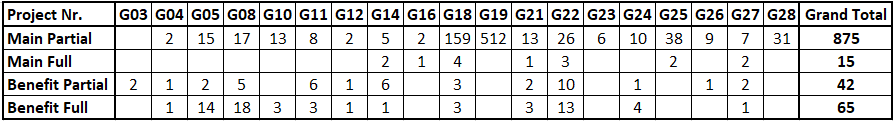
\includegraphics[scale=0.6]{Table/ground_truth.png}
	\captionof{table}{Detail about full and partial redundancies related to main or benefit parts as ground truth}\label{tb:ground_truth}
	
	\endgroup
\end{figure}
As we can see, the main parts of the US-pairs have less full redundancy (15 cases), which means that there are 15 cases where the main part of the US-pairs is exactly the same. This level of redundancy indicates common functionality of the US-pairs, which is a sign of overlapping features. 

A much higher occurrence of partial redundancy in the main parts(875 cases) indicates that there are common elements between the US-pairs, but still enough differences to avoid a complete match. 

Fewer instances of partial redundancy in the benefit parts (42 cases) indicate that the USs diverge in their benefit clauses, they are more tailored to specific project outcomes. 

The higher count of full redundancies (42 cases) compared to partial redundancies in the benefit parts is interesting, as it indicates that the expected objectives of certain features are often repeated in the USs. This suggests that the project is aiming for a set of common goals regardless of the specific functionality.
\subsubsection*{Evaluation of US Redundancy using Tool}
The automated tool is designed to identify redundancy among USs based on predefined criteria. It operates by analysing the text and structure of USs to detect similarities that could indicate redundancy.

In contrast to ground truth, which is based on one-to-one comparison of phrases in specific parts of USs, tool evaluation relies heavily on specified labelling (targets, triggers, contains) using the Doccano tool.

The following criteria are defined for the evaluation of US-pairs:
\begin{itemize}
	\item Full redundancy: 	A pair of US is considered to have "full redundancy" in the main or benefit part when every labelled clause in that part—comprising triggers (in the main part), targets, and contains—is syntactically identical.
	
	\item Partial redundancy: When only some labelled clauses, such as targets, have significant overlap but are not completely identical. This means that while certain labelled clauses, such as targets, may match between USs, other labelled clauses, such as triggers or contains, may differ, meaning that the USs are not fully redundant. This scenario suggests that while USs have significant similarities, they still contain unique aspects.
\end{itemize}
Table \ref{tb:tool} shows the aggregation of the full and partial redundancies in the main and benefit parts assessed by the tool. It is also worth noting that the numbers highlighted in red show the variation in the ground truth evaluation.
\begin{figure}[h]
	\begingroup
	\scriptsize
	\centering
	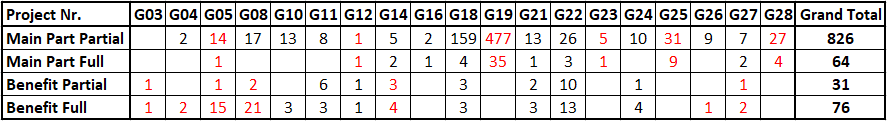
\includegraphics[scale=0.6]{Table/tool.png}
	\captionof{table}{Aggregation of the count of full and partial redundancies in relation to the main or benefit parts assessed by the tool}\label{tb:tool}
	\endgroup
\end{figure}
\paragraph{Assessment of Result: High-Level Overview}Based on the datasets provided, it was found that 1,851 redundancy clauses were identified across all projects, with the highest count found in the backlog G19 dataset (925 clauses), indicating a significant presence of redundancy in the USs of this project. 

Table \ref{tb:redundancy_clauses} shows the total number of redundancy clauses found in each dataset.
\begin{figure}[h]
	\begingroup
	\scriptsize
	\centering
	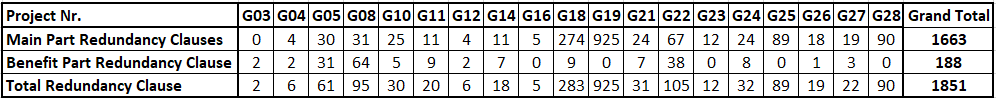
\includegraphics[scale=0.55]{Table/redundancy_clauses.png}
	\captionof{table}{Detail about number of redundancy clauses occurred in main and benefit parts}\label{tb:redundancy_clauses}
	
	\endgroup
\end{figure}
\paragraph{Assessment of Result: Aggregated Analysis}We also look for an aggregate for the count of redundant clauses in both the main and the benefit parts of the USs. 

In the main parts, the large count of full redundancies, especially where two clauses are present (6 clauses), indicates a high degree of similarity in the functionalities described.

In the benefit part of the USs, there is a considerable count of cases where full redundancy prevails, especially where two clauses are inserted (24 clauses). The large count of full redundancies with two clauses indicates that benefits are often described in a standardised way in the different USs.

Figure \ref{fig:aggregation} illustrates the aggregation of the count of redundancy clauses that occur in USs.

\begin{figure}[h]
	\centering
	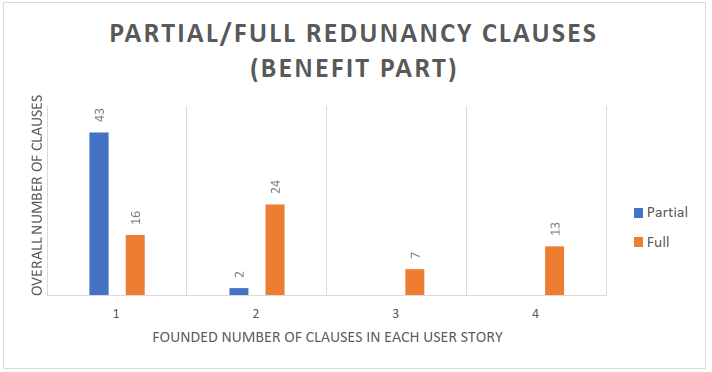
\includegraphics[scale=0.5]{aggregation_benefit}
	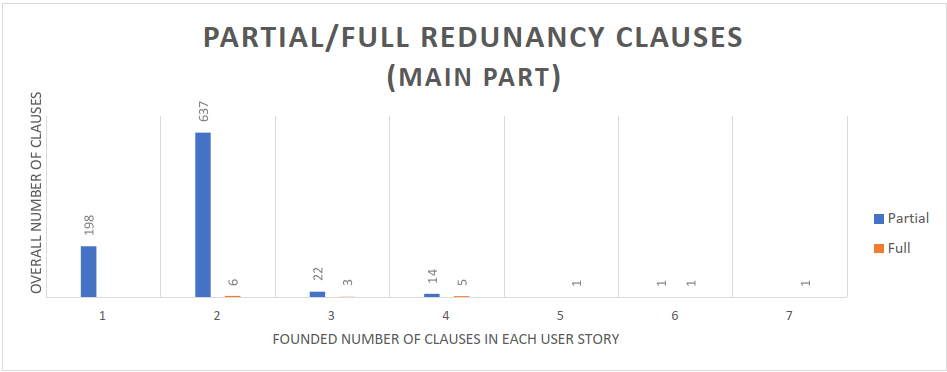
\includegraphics[scale=0.5]{aggregation_main}
	\caption{The aggregation between the count of redundancy clauses occurred in USs}\label{fig:aggregation}
\end{figure}
\paragraph{Assessment of Result: Detailed Insights}In the dataset of Backlog G19, the clause \enquote{have alfred} was repeated in all USs, indicating that \enquote{alfred} is the end product and not a specific functionality. This suggests that the quality of the USs should be considered, so that they do not contain generic information that results in a lot of redundant information(false positives) being provided.

In the main parts of the USs, 1,663 clauses were redundant("Main Part Redundancy Clauses" in Table \ref{tb:redundancy_clauses}), while only 188 redundancy clauses were found in the benefit parts("Benefit Part Redundancy Clauses" in Table \ref{tb:redundancy_clauses}). This means that some USs are not often written in a standardised format for the description of core functions, resulting in a higher count of redundant clauses in the main part.
\begin{example}
	In the dataset of backlog G18 (274 clauses out of 283 in the main parts), for example, this is due to the clauses \enquote{have ability} in the main part, which are unnecessarily repeated in most USs:\\
	\textit{user\_story\_92:} \#g18\# as a \#researcher\# I want to have \#the \#ability\# to search files by file type and format.\\
	\textit{user\_story\_80:} \#g18\# as a \#researcher\# I want to have \#the \#ability\# to attach standard metadata for behavioural observations (and video) so that my data can be searched and understood later.\\
	Actually, the clause \enquote{have ability} in USs should be deleted and no redundancy should be possible at all:\\
	\textit{user\_story\_92:} \#g18\# as a researcher I want to search for files by file type and format.\\
	\textit{user\_story\_80:} \#As a researcher, I want to attach standard metadata for behavioural observations (and videos), so that my data can be searched and understood later.
\end{example}

There are also USs with the same functionality, but one provides more details about the functionality. In other words, one US is contained within another, and we refer to them as full
redundant US-pairs, as deleting the US with less detail has no negative impact on the system. Sometimes it is necessary to merge these two USs to obtain a single detailed US.
\begin{example}
	In the dadaset of backlog G18, for example, we have two US-pairs that are marked as full redundancy between user\_story\_12 and user\_story\_11 as well as user\_story\_13 and user\_story\_11:\\
	\textit{user\_story\_12}: \enquote{\#g18\# as a \#researcher\#, I want to \#upload\# \#files\# prior to having them \#attached\# to a \#log book page\# using the web interface.}\\
	\textit{user\_story\_11:} \enquote{\#g18\# as a \#researcher\#, I want to \#upload\# \#files\# prior to having them \#attached\# to a \#log book page\#.}\\
	\textit{user\_story\_13:} \enquote{\#g18\# as a \#researcher\#, I want to \#upload\# \#files\# prior to having them \#attached\# to a \#log book page\# using a mapped network drive.}\\
	
	As we can see, the user\_story\_11 is an incomplete version of two other USs, and deleting it has no negative impact in the system, due to the fact that its goal is achieved and fulfilled by two other USs.
\end{example}
\paragraph{Research question 1: Conclusion}
After comparing the Ground Truth result with the result provided by our tool, the following realisation was made:
\begin{itemize}
	\item Main Part Partial: A -5.6\% (negative) percentage suggests that the Framework has fewer "Main Part Partial" counts than the Ground Truth.
	In this case, the Framework has about 5.6\% fewer "Main Part Partial" counts than expected.
	
	\item Main Part Full: A high positive percentage of 326.67\% indicates that the Framework has a significantly higher count of Main Part Full compared to Ground Truth.
	At 326.67\%, the framework has more than three times as many main part full compared to the ground truth.
	In our investigation, we found that some phrases are not included as relationship (contains or targets) in the USs annotated with the Doccano tool. Therefore, our tool categorised some USs as fully redundant when in reality they were only partially redundant.
	
	\item Count of Benefit Partial: -26.19\% a negative percentage here indicates that the Framework has fewer "Benefit Partial" counts compared to the Ground Truth.
	With -26.19\%, the Framework has approximately one-quarter fewer "Benefit Partial" counts.
	
	\item Count of Benefit Full: 16.92\% a positive percentage indicates that the Framework has more "Benefit Full" counts compared to the Ground Truth.
	With 16.92\%, the Framework has almost 17\% more "Benefit Full" counts than the Ground Truth.
\end{itemize}
It is also notable that if we add founded partial and full redundancies in main or benefit parts, we both amount are identical(main part: 890 cases , benefit part: 107).

This consistency indicates that the automated tool's results align with the ground truth, suggesting that the tool is reliable in detecting redundancy. It demonstrates that the tool's performance closely matches the personal assessment, reinforcing confidence in its accuracy and validity.
\subsubsection*{Performance Evaluation}
To answer the second research question "How does the tool's performance scale as the count of USs in a backlog increases?", we conducted a series of tests to measure the time it takes the tool to process different counts of USs. This section describes the testing methodology, the results obtained and the impact on the scalability of the tool.
\paragraph{Test Methodology}To evaluate the tool's performance, we conducted a set of experiments in which the tool processed different numbers of USs in a backlog. The tests involved the following steps:
\begin{enumerate}
	\item Backlog Setup: We used backlogs with varying numbers of USs around—50, 70, 90, 120 and 140—to simulate different workload sizes. Each backlog contained USs with varying content, redundancy elements, and complexity to represent a realistic range of cases. Table \ref{tb:performance_env} shows information on the backlog data records provided for the performance test application.
	\begin{figure}[h]
		\begingroup
		\scriptsize
		\centering
		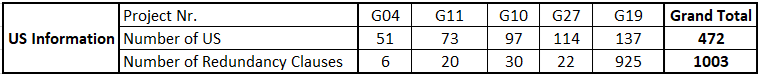
\includegraphics[scale=0.7]{Table/performance_env.png}
		\captionof{table}{Information on the backlog datasets provided for the application of the performance test}\label{tb:performance_env}
		\endgroup
	\end{figure}
	\item Tool Execution: Each part of toolchain(Rule creation, CDA tool, report creation and evaluation) was run for each backlog and the total time taken to process the entire backlog was recorded. The performance of the tool was measured by the processing time, i.e. the total time taken to process all USs in the backlog and identify redundancies.
	
	\item Repeating Tests: To ensure reliability, each test was conducted multiple times, and the average processing time was calculated.
\end{enumerate}
The test environment consisted of:
\begin{itemize}
	\item Processor: Intel(R) Core(TM) i7-8565U CPU @ 1.80GHz (8 CPUs), ~2.0GHz		
	\item Memory: 8070MB RAM
	\item Display Devices: Intel(R) UHD Graphics 620, 4163 MB(Display Memory)
	\item Hard Disk: INTEL SSDPEKNW512G8H
	\item Operating System: Windows 11 Home 64-bit (10.0, Build 22631) (22621.ni\_release.220506-1250)
	\item System Type: 64-bit operating system, x64-based processor
\end{itemize}
Table \ref{tb:performance_result} shows the result of tool's performance in seconds which were conducted on a controlled environment to ensure consistency.

	\begin{figure}[h]
	\begingroup
	\scriptsize
	\centering
	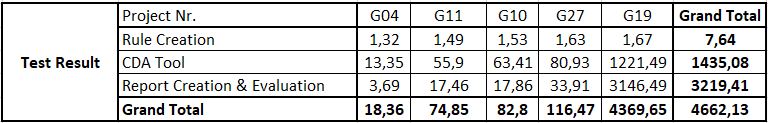
\includegraphics[scale=0.7]{Table/performance_result.png}
	\captionof{table}{Information about the result of the tool's performance test, which was measured using the processing time in seconds.}\label{tb:performance_result}
	\endgroup
\end{figure}
\paragraph{Research question 2: Conclusion}As we can see, there is a direct correlation between the number of USs in a backlog and the time our tool needs to process them. The results confirm that developers and project managers should expect a longer processing time when evaluating redundancy as the backlog grows.

However, the impact on processing time varies depending on the process in question. While rule creation using the Henshin API shows relatively consistent and lower processing times, other components such as the CDA tool and report creation processes show an exponential increase in processing time as the number of USs increases. This indicates that certain processes scale differently as the data load increases.

An important observation is that with a larger number of USs, the probability of finding redundant clauses between USs increases. This has a significant impact on redundancy detection and backlog management specially during processing of CDA tool. As the data set grows, there are more opportunities for overlaps, repetitions or similar USs that could indicate redundancy.
\subsubsection*{Threats to Validity}
When assessing the redundancy of USs through both personal assessment (ground truth) and the automated tool, several potential threats to validity must be considered. This section outlines the main threats to validity and describes how they were mitigated during the study.
\paragraph{Construct validity}It refers to the extent to which the assessment measures what it is intended to measure. The following risks were identified:
\begin{itemize}
	\item Ambiguity of criteria: If the criteria for redundancy are unclear or open to interpretation, this can lead to inconsistent scores. To avoid this, we defined clear and detailed criteria for identifying redundancy in USs.
	
	\item Subjectivity in ground truth: As ground truth is based on personal judgement, subjectivity could lead to bias. To minimise this risk, we cross-checked out evaluations with another experienced evaluator.
\end{itemize}
\paragraph{External validity}External validity refers to the generalisability of the study results to other contexts or population groups. Threats to external validity include:

\begin{itemize}
	\item specificity of USs: If the USs used in the study are too specific or context-dependent, the results may not be transferable to other projects. To mitigate this, we included 19 backlog datasets with different USs and different project types in the analysis.
	
	\item Tool Limitation: The automated tool is designed for a specific format of USs, which limits its broader applicability. Our tool depends heavily on the specific US's format (e.g. "As a \textless user\textgreater, I want to ..., so that..."), which is essential for the application of the tool. Therefore, we tested the tool in isolated contexts limited to well-formed USs and analysed its performance in a number of scenarios.
	
	Another limitation is that our tool is dependent on the specific type of annotation used for USs. In our case, these are annotations such as action, entity, their reference targets, triggers and contains. This means that the effectiveness of the tool depends on the accuracy and consistency of these annotations. If the annotations are incomplete or incorrect, the tool may not work as expected. In addition, the tool may not be compatible with other annotation schemes that do not use these specific labels.
\end{itemize}
\paragraph{Internal Validity}Internal validity is concerned with whether the observed results are attributable to the factors analysed or are influenced by other variables. Potential threats to internal validity include:
\begin{itemize}
	\item Confounding factors: External influences or unintended variables could influence the assessment of redundancy. In particular, USs annotated with Doccano are a very critical impact when evaluating full and partial redundancies between USs using tool. The more phrases are covered in the relationship(targets, contains), the better the score. Since our tool uses Doccano annotated USs as primary input without any changes, these discrepancies are unavoidable. % To avoid this, I controlled the scope of the study to ensure that all user reports came from a consistent context and that consistent evaluation methods were used.
	
	\item Limitation of tool: The automated tool may not capture all aspects of redundancy, especially semantically. This leads us to the next step, the semantic analysis of USs.
\end{itemize}
\subsection{Conclusion}\label{redundancy_conclustion}
In this study, we developed and applied a comprehensive approach that combines the Doccano tool, Henshin and the CDA tool to systematically identify and report redundancies in USs within software development projects with an evaluation.

By carefully analysing 19 different backlog datasets, our method not only separated USs into main and benefit parts for nuanced examination, but also facilitated the distinction between full and partial redundancies within these parts.

Our results reveal a crucial finding: the effectiveness of redundancy detection is significantly influenced by the quality of the USs as well as annotated USs. Well-formulated USs that do not contain unnecessary clauses (e.g. the repetition of \enquote{end product} in all USs) and a concisely annotated backlog specially in relation properties also have a major influence on the effective redundancy analysis process.

 If the main part is evaluated to be full redundant, then we have a US-pair that is functionally identical and we can merge the US-pair into one US. In the case of full redundancy in the benefit part, this means that the US-pairs belong to the same goal and objective, to which they should be categorised for better accessibility and understanding.
 
A notable trend emerged from our analysis: the benefit parts are more often fully redundant than the main parts of USs. This indicates that multiple USs often strive for different functions that contribute to a common system aspect or goal.

Recognising such redundancies not only helps to consolidate functionally identical US-pairs into single, more compact USs, but also to group US-pairs together, improving accessibility and understanding of project backlogs.

In summary, our study confirms the central role of a syntactic analysis approach in detecting and managing redundancies in project backlogs, thereby contributing to the rationalisation of software development processes.

While the quality of annotated USs plays a critical role in the success of this approach, the insights gained from this research provide valuable guidance for both current practices and future research in software project management.

However, our investigation has also shown that we can only consider USs with syntactic redundancy. If they are indeed US-pairs with the same functionality but using different words and clauses to achieve the same goal, we cannot detect this with this approach.

This finding shows that the distinction between actual redundancy and mere superficial similarity can be further refined, which leads us to analyse the USs semantically.

In the next section, we therefore present a method for analysing conflicts and dependencies between USs in semantic way.
%We also find that there are more full redundancy in the benefit part as compared to main part, as the USs with the same benefit achieve different functions for the same aspect of system.

%We have realised that some user stories are only apparently part of other USs, so we can merge them into a compact single US.
%\subsection{Evaluation}\label{redundancy_evaluation}
%In this section we will present the results of applying our approach to analyse USs in 19 by CRF tool annotated backlog datasets. 
%The purpose of this section is to assess the effectiveness of our approach in analysing redundancy between USs. This section serves several key objective:
In this section, we address two different research questions and provide a detailed explanation of the experimental design and execution for each question. We also present a detailed analysis of the results to provide answers to these research questions, highlight their implications and provide insights into the research findings.
%\begin{itemize}
%	\item Demonstrating the validity and reliability of our proposed methodology for identifying and categorising redundancies between USs.
%	\item Presenting the results of our analysis across multiple datasets, highlighting the prevalence of \enquote{Full and Partial Redundancy} for both the main and benefit parts of USs.
%	\item Gaining insights into the nature and extent of redundancies between USs and its potential impact on software development processes.
%	\item Comparing results from different data sets, identifying patterns or trends and analysing variations in redundancy levels.
%\end{itemize}
\subsubsection*{Research Questions}
The research questions addressed in this section are as follows:
\begin{enumerate}
	\item Does our tool reliably determine the level of redundancy —either partial or full— between different parts of USs (main and benefit)?
	\item How does the tool's performance scale when the number of USs in a backlog increases?
	\end{enumerate}
\subsubsection*{Methodology}
To address the first questions "Does our tool reliably determine the level of redundancy—either partial or full—between different parts of USs (main and benefit)?", we recap the methodology employed to analyse redundancy between USs. We utilized a systematic approach that involved several key steps:
\begin{itemize}
	
	\item Data Collection: For a comprehensive assessment, we applied our approach to 19 backlog datasets presented by Mosser et al.\footnote{https://github.com/ace-design/nlp-stories}. They applied the Doccano approach to these publicly available requirements datasets\cite{requirementsdatasets}.
	
	It is also worth noting that some backlog datasets (g02, g13, g17, g27) did not follow the expected sentence structure, which is why we did not include them in the evaluation results to avoid unexpected behaviour. Table \ref{tb:backlogs} shows the project number of each dataset and the count of USs.
	%	- You have to describe all that in your work, how do you define Main Partial/Full and Benefit Partial/Full, so how do you decide that. And generating this JSON_Report and filling this table is all interesting implementation information.
	
	%When evaluating, I use tools on a large scale and I go through all the cases and look at what comes out of the use case as a meaningful result. As an evaluation, I will enter all the datasets we have as input and then what comes out will be 
	\begingroup
	\centering
	\scriptsize
	\renewcommand{\arraystretch}{1.5} 
	%\keepXColumns
	\begin{tabularx}{\linewidth}{l|XXXXXXXXXXXXXXXXXXX|X}
		Item&	1&	2&	3&	4&	5&	6&	7&	8&	9&	10&	11&	12&	13&	14&	15&	16&	17&	18&	19&	\\
		\hline
		%Project Name&loudoun&recycling&openspending&frictionless&scrumalliance	&nsf&camperplus&datahub&mis&neurohub&alfred&badcamp&rdadmp&archivesspace	&unibath&duraspace&racdam&culrepo&zooniverse&\\
		Project Nr.&	g03	&g04	&g05	&g08	&g10	&g11	&g12	&g14	&g16	&g18	&g19	&g21	&g22	&g23	&g24	&g25	&g26	&g27	&g28	&Total USs\\
		\hline
		Total USs&	57&	51	&53	&66	&97	&73	&54	&67	&66	&102	&137	&69	&83	&56	&53	&100	&100	&114	&60	&1458 \\
		\caption{Project number and count of USs contained in each backlog dataset}\label{tb:backlogs}
	\end{tabularx}	
	\endgroup
	
	%\item Preprocessing: Using the generated JSON report file for each dataset, we create a VBA script called \textit{extractFromJSONFiles}\footnote{https://github.com/amirrabieyannejad/USs\_Annotation/tree/main/Skript/extractFromJSONFiles} to iterate through all the JSON report files and extract the information such as \enquote{US-pair}, \enquote{US-text}, \enquote{total redundancy clauses}, \enquote{main redundancy clauses}, \enquote{benefit redundancy clauses} and \enquote{project number} and collect them all in an Excel file to perform further analyses.
	
	\item Identification of main and benefit parts: Each US was divided into its main part, which is the core functionality, and its benefit part, which describes the value to the persona.
	
	\item Detection of overlapping clauses: Recognition of overlapping clauses between a US-pair in a specific part of the USs.
	
	\item Redundancy analysis in main and benefit parts: Based on the redundant clauses identified, an automatic redundancy analysis was performed for the main and benefit parts of the US-pair based on certain criteria indicating the level of redundancy (partial or full) in the main and benefit parts.
		
	%\item Preprocessing: \item preprocessing: We transform each data set into graph transformation rules, apply CDA and generate a textual report in which each redundancy clause between US-pairs is marked with a hash symbol. Additionally,  the number of founded redundancies in the main and benefit sections is also determined.
\end{itemize}
\subsubsection*{Ground Truth Evaluation of US Redundancy}
Answering the first research question requires our automated system to have a reference point against which its accuracy can be measured. This reference point or "ground truth" is derived from a personal assessment and serves as a benchmark for the tool's performance.

In contrast to the tool evaluation, we did not evaluate based on labels (e.g., action, entity, persona, targets, etc.) in the personal evaluation. This means that when evaluating ground truth, we evaluate partial and full redundancy based on the phrases occurring in a given part as a one-to-one comparison.

The ground truth is the final assessment against which automated results are compared. It is derived from the personal judgement of a subject matter expert (in this case myself) using a combination of expertise, experience and specific evaluation criteria. The personal assessment is targeted at providing a reliable and accurate reference for redundancy between USs.\\\\
	The following criteria were taken into account in the personal assessment:
	\begin{itemize}
		\item A US-pair is evaluated as fully redundant in the main part, if all phrases occurred in the main parts of both USs fully overlap with one-to-one comparison. For example, the following US-pair is assessed as fully redundant:\\
		user\_story\_01: "\#g14\# as a \#publisher\#, i want to \#publish\# a \#dataset\#, so that i can view just the dataset with a few people."
		
		user\_story\_02: "\#g14\# as a \#publisher\#, i want to \#publish\# a \#dataset\#, so that i can share the dataset publicly with everyone."
		
		\item A US-pair is considered fully redundant in the main part, if all phrases in the main part of at least one US completely overlap. For instance:\\
		user\_story\_22: "\#g14\# as a \#consumer\#, i want to \#view\# a \#data package\# online, so that i can \#get\# a \#sense\# of whether this is the dataset i want."
		
		user\_story\_24: "\#g14\# as a \#consumer\#, i want to \#view\# the \#data package\#, so that that i can \#get\# a \#sense\# of whether i want this dataset or not."
		
		\item A US-pair is categorised as partially redundant in the main part if some phrases remain distinctive between the USs. For Instance:\\
		user\_story\_09: "\#g04\# as a \#user\#, i want to be able to \#view\# a \#map display\# of the public recycling bins around my \#area\#."
		
		user\_story\_10: "\#g04\# as a \#user\#, i want to be able to \#view\# a \#map display\# of the special waste drop off sites around my \#area\#."
		
		\item The criteria mentioned were also applied to the benefit part.
	\end{itemize}
Table \ref{tb:ground_truth} shows the aggregation of full and partial redundancies in the main and benefit parts as ground truth.
\begin{figure}[h]
	\begingroup
	\scriptsize
	\centering
	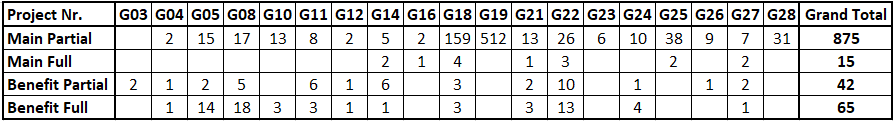
\includegraphics[scale=0.6]{Table/ground_truth.png}
	\captionof{table}{Detail about full and partial redundancies related to main or benefit parts as ground truth}\label{tb:ground_truth}
	
	\endgroup
\end{figure}
As we can see, the main parts of the US-pairs have less full redundancy (15 cases), which means that there are 15 cases where the main part of the US-pairs is exactly the same. This level of redundancy indicates common functionality of the US-pairs, which is a sign of overlapping features. 

A much higher occurrence of partial redundancy in the main parts(875 cases) indicates that there are common elements between the US-pairs, but still enough differences to avoid a complete match. 

Fewer instances of partial redundancy in the benefit parts (42 cases) indicate that the USs diverge in their benefit clauses, they are more tailored to specific project outcomes. 

The higher count of full redundancies (42 cases) compared to partial redundancies in the benefit parts is interesting, as it indicates that the expected objectives of certain features are often repeated in the USs. This suggests that the project is aiming for a set of common goals regardless of the specific functionality.
\subsubsection*{Evaluation of US Redundancy using Tool}
The automated tool is designed to identify redundancy among USs based on predefined criteria. It operates by analysing the text and structure of USs to detect similarities that could indicate redundancy.

In contrast to ground truth, which is based on one-to-one comparison of phrases in specific parts of USs, tool evaluation relies heavily on specified labelling (targets, triggers, contains) using the Doccano tool.

The following criteria are defined for the evaluation of US-pairs:
\begin{itemize}
	\item Full redundancy: 	A pair of US is considered to have "full redundancy" in the main or benefit part when every labelled clause in that part—comprising triggers (in the main part), targets, and contains—is syntactically identical.
	
	\item Partial redundancy: When only some labelled clauses, such as targets, have significant overlap but are not completely identical. This means that while certain labelled clauses, such as targets, may match between USs, other labelled clauses, such as triggers or contains, may differ, meaning that the USs are not fully redundant. This scenario suggests that while USs have significant similarities, they still contain unique aspects.
\end{itemize}
Table \ref{tb:tool} shows the aggregation of the full and partial redundancies in the main and benefit parts assessed by the tool. It is also worth noting that the numbers highlighted in red show the variation in the ground truth evaluation.
\begin{figure}[h]
	\begingroup
	\scriptsize
	\centering
	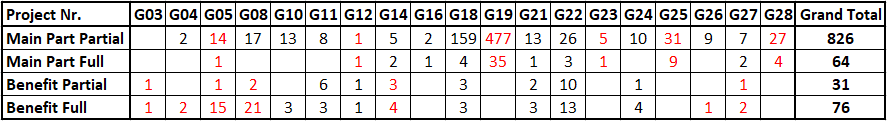
\includegraphics[scale=0.6]{Table/tool.png}
	\captionof{table}{Aggregation of the count of full and partial redundancies in relation to the main or benefit parts assessed by the tool}\label{tb:tool}
	\endgroup
\end{figure}
\paragraph{Assessment of Result: High-Level Overview}Based on the datasets provided, it was found that 1,851 redundancy clauses were identified across all projects, with the highest count found in the backlog G19 dataset (925 clauses), indicating a significant presence of redundancy in the USs of this project. 

Table \ref{tb:redundancy_clauses} shows the total number of redundancy clauses found in each dataset.
\begin{figure}[h]
	\begingroup
	\scriptsize
	\centering
	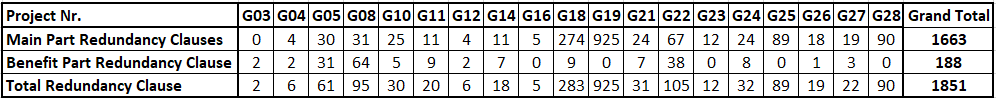
\includegraphics[scale=0.55]{Table/redundancy_clauses.png}
	\captionof{table}{Detail about number of redundancy clauses occurred in main and benefit parts}\label{tb:redundancy_clauses}
	
	\endgroup
\end{figure}
\paragraph{Assessment of Result: Aggregated Analysis}We also look for an aggregate for the count of redundant clauses in both the main and the benefit parts of the USs. 

In the main parts, the large count of full redundancies, especially where two clauses are present (6 clauses), indicates a high degree of similarity in the functionalities described.

In the benefit part of the USs, there is a considerable count of cases where full redundancy prevails, especially where two clauses are inserted (24 clauses). The large count of full redundancies with two clauses indicates that benefits are often described in a standardised way in the different USs.

Figure \ref{fig:aggregation} illustrates the aggregation of the count of redundancy clauses that occur in USs.

\begin{figure}[h]
	\centering
	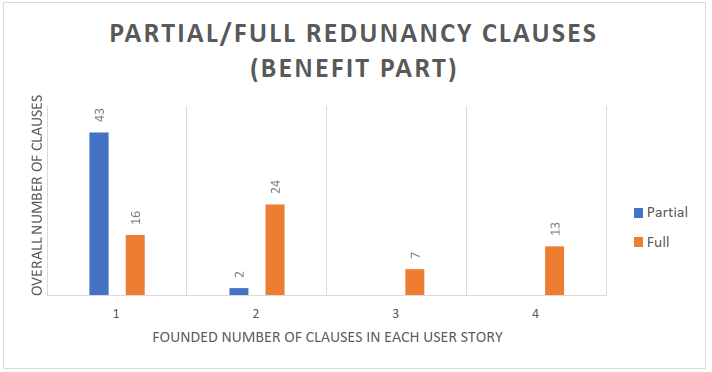
\includegraphics[scale=0.5]{aggregation_benefit}
	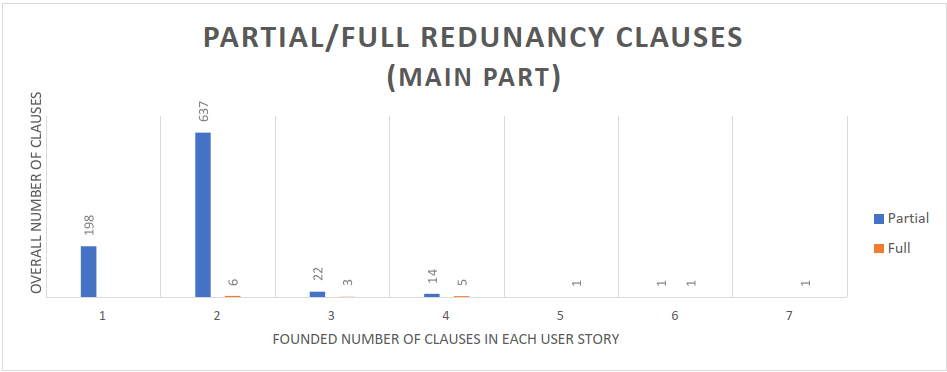
\includegraphics[scale=0.5]{aggregation_main}
	\caption{The aggregation between the count of redundancy clauses occurred in USs}\label{fig:aggregation}
\end{figure}
\paragraph{Assessment of Result: Detailed Insights}In the dataset of Backlog G19, the clause \enquote{have alfred} was repeated in all USs, indicating that \enquote{alfred} is the end product and not a specific functionality. This suggests that the quality of the USs should be considered, so that they do not contain generic information that results in a lot of redundant information(false positives) being provided.

In the main parts of the USs, 1,663 clauses were redundant("Main Part Redundancy Clauses" in Table \ref{tb:redundancy_clauses}), while only 188 redundancy clauses were found in the benefit parts("Benefit Part Redundancy Clauses" in Table \ref{tb:redundancy_clauses}). This means that some USs are not often written in a standardised format for the description of core functions, resulting in a higher count of redundant clauses in the main part.
\begin{example}
	In the dataset of backlog G18 (274 clauses out of 283 in the main parts), for example, this is due to the clauses \enquote{have ability} in the main part, which are unnecessarily repeated in most USs:\\
	\textit{user\_story\_92:} \#g18\# as a \#researcher\# I want to have \#the \#ability\# to search files by file type and format.\\
	\textit{user\_story\_80:} \#g18\# as a \#researcher\# I want to have \#the \#ability\# to attach standard metadata for behavioural observations (and video) so that my data can be searched and understood later.\\
	Actually, the clause \enquote{have ability} in USs should be deleted and no redundancy should be possible at all:\\
	\textit{user\_story\_92:} \#g18\# as a researcher I want to search for files by file type and format.\\
	\textit{user\_story\_80:} \#As a researcher, I want to attach standard metadata for behavioural observations (and videos), so that my data can be searched and understood later.
\end{example}

There are also USs with the same functionality, but one provides more details about the functionality. In other words, one US is contained within another, and we refer to them as full
redundant US-pairs, as deleting the US with less detail has no negative impact on the system. Sometimes it is necessary to merge these two USs to obtain a single detailed US.
\begin{example}
	In the dadaset of backlog G18, for example, we have two US-pairs that are marked as full redundancy between user\_story\_12 and user\_story\_11 as well as user\_story\_13 and user\_story\_11:\\
	\textit{user\_story\_12}: \enquote{\#g18\# as a \#researcher\#, I want to \#upload\# \#files\# prior to having them \#attached\# to a \#log book page\# using the web interface.}\\
	\textit{user\_story\_11:} \enquote{\#g18\# as a \#researcher\#, I want to \#upload\# \#files\# prior to having them \#attached\# to a \#log book page\#.}\\
	\textit{user\_story\_13:} \enquote{\#g18\# as a \#researcher\#, I want to \#upload\# \#files\# prior to having them \#attached\# to a \#log book page\# using a mapped network drive.}\\
	
	As we can see, the user\_story\_11 is an incomplete version of two other USs, and deleting it has no negative impact in the system, due to the fact that its goal is achieved and fulfilled by two other USs.
\end{example}
\paragraph{Research question 1: Conclusion}
After comparing the Ground Truth result with the result provided by our tool, the following realisation was made:
\begin{itemize}
	\item Main Part Partial: A -5.6\% (negative) percentage suggests that the Framework has fewer "Main Part Partial" counts than the Ground Truth.
	In this case, the Framework has about 5.6\% fewer "Main Part Partial" counts than expected.
	
	\item Main Part Full: A high positive percentage of 326.67\% indicates that the Framework has a significantly higher count of Main Part Full compared to Ground Truth.
	At 326.67\%, the framework has more than three times as many main part full compared to the ground truth.
	In our investigation, we found that some phrases are not included as relationship (contains or targets) in the USs annotated with the Doccano tool. Therefore, our tool categorised some USs as fully redundant when in reality they were only partially redundant.
	
	\item Count of Benefit Partial: -26.19\% a negative percentage here indicates that the Framework has fewer "Benefit Partial" counts compared to the Ground Truth.
	With -26.19\%, the Framework has approximately one-quarter fewer "Benefit Partial" counts.
	
	\item Count of Benefit Full: 16.92\% a positive percentage indicates that the Framework has more "Benefit Full" counts compared to the Ground Truth.
	With 16.92\%, the Framework has almost 17\% more "Benefit Full" counts than the Ground Truth.
\end{itemize}
It is also notable that if we add founded partial and full redundancies in main or benefit parts, we both amount are identical(main part: 890 cases , benefit part: 107).

This consistency indicates that the automated tool's results align with the ground truth, suggesting that the tool is reliable in detecting redundancy. It demonstrates that the tool's performance closely matches the personal assessment, reinforcing confidence in its accuracy and validity.
\subsubsection*{Performance Evaluation}
To answer the second research question "How does the tool's performance scale as the count of USs in a backlog increases?", we conducted a series of tests to measure the time it takes the tool to process different counts of USs. This section describes the testing methodology, the results obtained and the impact on the scalability of the tool.
\paragraph{Test Methodology}To evaluate the tool's performance, we conducted a set of experiments in which the tool processed different numbers of USs in a backlog. The tests involved the following steps:
\begin{enumerate}
	\item Backlog Setup: We used backlogs with varying numbers of USs around—50, 70, 90, 120 and 140—to simulate different workload sizes. Each backlog contained USs with varying content, redundancy elements, and complexity to represent a realistic range of cases. Table \ref{tb:performance_env} shows information on the backlog data records provided for the performance test application.
	\begin{figure}[h]
		\begingroup
		\scriptsize
		\centering
		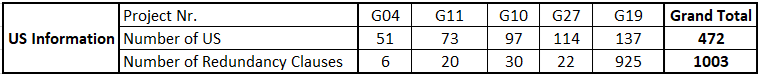
\includegraphics[scale=0.7]{Table/performance_env.png}
		\captionof{table}{Information on the backlog datasets provided for the application of the performance test}\label{tb:performance_env}
		\endgroup
	\end{figure}
	\item Tool Execution: Each part of toolchain(Rule creation, CDA tool, report creation and evaluation) was run for each backlog and the total time taken to process the entire backlog was recorded. The performance of the tool was measured by the processing time, i.e. the total time taken to process all USs in the backlog and identify redundancies.
	
	\item Repeating Tests: To ensure reliability, each test was conducted multiple times, and the average processing time was calculated.
\end{enumerate}
The test environment consisted of:
\begin{itemize}
	\item Processor: Intel(R) Core(TM) i7-8565U CPU @ 1.80GHz (8 CPUs), ~2.0GHz		
	\item Memory: 8070MB RAM
	\item Display Devices: Intel(R) UHD Graphics 620, 4163 MB(Display Memory)
	\item Hard Disk: INTEL SSDPEKNW512G8H
	\item Operating System: Windows 11 Home 64-bit (10.0, Build 22631) (22621.ni\_release.220506-1250)
	\item System Type: 64-bit operating system, x64-based processor
\end{itemize}
Table \ref{tb:performance_result} shows the result of tool's performance in seconds which were conducted on a controlled environment to ensure consistency.

	\begin{figure}[h]
	\begingroup
	\scriptsize
	\centering
	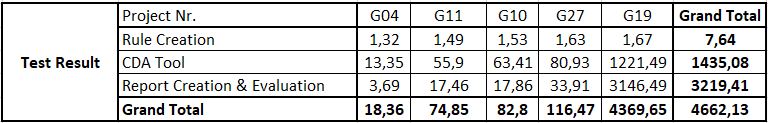
\includegraphics[scale=0.7]{Table/performance_result.png}
	\captionof{table}{Information about the result of the tool's performance test, which was measured using the processing time in seconds.}\label{tb:performance_result}
	\endgroup
\end{figure}
\paragraph{Research question 2: Conclusion}As we can see, there is a direct correlation between the number of USs in a backlog and the time our tool needs to process them. The results confirm that developers and project managers should expect a longer processing time when evaluating redundancy as the backlog grows.

However, the impact on processing time varies depending on the process in question. While rule creation using the Henshin API shows relatively consistent and lower processing times, other components such as the CDA tool and report creation processes show an exponential increase in processing time as the number of USs increases. This indicates that certain processes scale differently as the data load increases.

An important observation is that with a larger number of USs, the probability of finding redundant clauses between USs increases. This has a significant impact on redundancy detection and backlog management specially during processing of CDA tool. As the data set grows, there are more opportunities for overlaps, repetitions or similar USs that could indicate redundancy.
\subsubsection*{Threats to Validity}
When assessing the redundancy of USs through both personal assessment (ground truth) and the automated tool, several potential threats to validity must be considered. This section outlines the main threats to validity and describes how they were mitigated during the study.
\paragraph{Construct validity}It refers to the extent to which the assessment measures what it is intended to measure. The following risks were identified:
\begin{itemize}
	\item Ambiguity of criteria: If the criteria for redundancy are unclear or open to interpretation, this can lead to inconsistent scores. To avoid this, we defined clear and detailed criteria for identifying redundancy in USs.
	
	\item Subjectivity in ground truth: As ground truth is based on personal judgement, subjectivity could lead to bias. To minimise this risk, we cross-checked out evaluations with another experienced evaluator.
\end{itemize}
\paragraph{External validity}External validity refers to the generalisability of the study results to other contexts or population groups. Threats to external validity include:

\begin{itemize}
	\item specificity of USs: If the USs used in the study are too specific or context-dependent, the results may not be transferable to other projects. To mitigate this, we included 19 backlog datasets with different USs and different project types in the analysis.
	
	\item Tool Limitation: The automated tool is designed for a specific format of USs, which limits its broader applicability. Our tool depends heavily on the specific US's format (e.g. "As a \textless user\textgreater, I want to ..., so that..."), which is essential for the application of the tool. Therefore, we tested the tool in isolated contexts limited to well-formed USs and analysed its performance in a number of scenarios.
	
	Another limitation is that our tool is dependent on the specific type of annotation used for USs. In our case, these are annotations such as action, entity, their reference targets, triggers and contains. This means that the effectiveness of the tool depends on the accuracy and consistency of these annotations. If the annotations are incomplete or incorrect, the tool may not work as expected. In addition, the tool may not be compatible with other annotation schemes that do not use these specific labels.
\end{itemize}
\paragraph{Internal Validity}Internal validity is concerned with whether the observed results are attributable to the factors analysed or are influenced by other variables. Potential threats to internal validity include:
\begin{itemize}
	\item Confounding factors: External influences or unintended variables could influence the assessment of redundancy. In particular, USs annotated with Doccano are a very critical impact when evaluating full and partial redundancies between USs using tool. The more phrases are covered in the relationship(targets, contains), the better the score. Since our tool uses Doccano annotated USs as primary input without any changes, these discrepancies are unavoidable. % To avoid this, I controlled the scope of the study to ensure that all user reports came from a consistent context and that consistent evaluation methods were used.
	
	\item Limitation of tool: The automated tool may not capture all aspects of redundancy, especially semantically. This leads us to the next step, the semantic analysis of USs.
\end{itemize}
\subsection{Conclusion}\label{redundancy_conclustion}
In this study, we developed and applied a comprehensive approach that combines the Doccano tool, Henshin and the CDA tool to systematically identify and report redundancies in USs within software development projects with an evaluation.

By carefully analysing 19 different backlog datasets, our method not only separated USs into main and benefit parts for nuanced examination, but also facilitated the distinction between full and partial redundancies within these parts.

Our results reveal a crucial finding: the effectiveness of redundancy detection is significantly influenced by the quality of the USs as well as annotated USs. Well-formulated USs that do not contain unnecessary clauses (e.g. the repetition of \enquote{end product} in all USs) and a concisely annotated backlog specially in relation properties also have a major influence on the effective redundancy analysis process.

 If the main part is evaluated to be full redundant, then we have a US-pair that is functionally identical and we can merge the US-pair into one US. In the case of full redundancy in the benefit part, this means that the US-pairs belong to the same goal and objective, to which they should be categorised for better accessibility and understanding.
 
A notable trend emerged from our analysis: the benefit parts are more often fully redundant than the main parts of USs. This indicates that multiple USs often strive for different functions that contribute to a common system aspect or goal.

Recognising such redundancies not only helps to consolidate functionally identical US-pairs into single, more compact USs, but also to group US-pairs together, improving accessibility and understanding of project backlogs.

In summary, our study confirms the central role of a syntactic analysis approach in detecting and managing redundancies in project backlogs, thereby contributing to the rationalisation of software development processes.

While the quality of annotated USs plays a critical role in the success of this approach, the insights gained from this research provide valuable guidance for both current practices and future research in software project management.

However, our investigation has also shown that we can only consider USs with syntactic redundancy. If they are indeed US-pairs with the same functionality but using different words and clauses to achieve the same goal, we cannot detect this with this approach.

This finding shows that the distinction between actual redundancy and mere superficial similarity can be further refined, which leads us to analyse the USs semantically.

In the next section, we therefore present a method for analysing conflicts and dependencies between USs in semantic way.
%We also find that there are more full redundancy in the benefit part as compared to main part, as the USs with the same benefit achieve different functions for the same aspect of system.

%We have realised that some user stories are only apparently part of other USs, so we can merge them into a compact single US.
%\subsection{Evaluation}\label{redundancy_evaluation}
%In this section we will present the results of applying our approach to analyse USs in 19 by CRF tool annotated backlog datasets. 
%The purpose of this section is to assess the effectiveness of our approach in analysing redundancy between USs. This section serves several key objective:
In this section, we address two different research questions and provide a detailed explanation of the experimental design and execution for each question. We also present a detailed analysis of the results to provide answers to these research questions, highlight their implications and provide insights into the research findings.
%\begin{itemize}
%	\item Demonstrating the validity and reliability of our proposed methodology for identifying and categorising redundancies between USs.
%	\item Presenting the results of our analysis across multiple datasets, highlighting the prevalence of \enquote{Full and Partial Redundancy} for both the main and benefit parts of USs.
%	\item Gaining insights into the nature and extent of redundancies between USs and its potential impact on software development processes.
%	\item Comparing results from different data sets, identifying patterns or trends and analysing variations in redundancy levels.
%\end{itemize}
\subsubsection*{Research Questions}
The research questions addressed in this section are as follows:
\begin{enumerate}
	\item Does our tool reliably determine the level of redundancy —either partial or full— between different parts of USs (main and benefit)?
	\item How does the tool's performance scale when the number of USs in a backlog increases?
	\end{enumerate}
\subsubsection*{Methodology}
To address the first questions "Does our tool reliably determine the level of redundancy—either partial or full—between different parts of USs (main and benefit)?", we recap the methodology employed to analyse redundancy between USs. We utilized a systematic approach that involved several key steps:
\begin{itemize}
	
	\item Data Collection: For a comprehensive assessment, we applied our approach to 19 backlog datasets presented by Mosser et al.\footnote{https://github.com/ace-design/nlp-stories}. They applied the Doccano approach to these publicly available requirements datasets\cite{requirementsdatasets}.
	
	It is also worth noting that some backlog datasets (g02, g13, g17, g27) did not follow the expected sentence structure, which is why we did not include them in the evaluation results to avoid unexpected behaviour. Table \ref{tb:backlogs} shows the project number of each dataset and the count of USs.
	%	- You have to describe all that in your work, how do you define Main Partial/Full and Benefit Partial/Full, so how do you decide that. And generating this JSON_Report and filling this table is all interesting implementation information.
	
	%When evaluating, I use tools on a large scale and I go through all the cases and look at what comes out of the use case as a meaningful result. As an evaluation, I will enter all the datasets we have as input and then what comes out will be 
	\begingroup
	\centering
	\scriptsize
	\renewcommand{\arraystretch}{1.5} 
	%\keepXColumns
	\begin{tabularx}{\linewidth}{l|XXXXXXXXXXXXXXXXXXX|X}
		Item&	1&	2&	3&	4&	5&	6&	7&	8&	9&	10&	11&	12&	13&	14&	15&	16&	17&	18&	19&	\\
		\hline
		%Project Name&loudoun&recycling&openspending&frictionless&scrumalliance	&nsf&camperplus&datahub&mis&neurohub&alfred&badcamp&rdadmp&archivesspace	&unibath&duraspace&racdam&culrepo&zooniverse&\\
		Project Nr.&	g03	&g04	&g05	&g08	&g10	&g11	&g12	&g14	&g16	&g18	&g19	&g21	&g22	&g23	&g24	&g25	&g26	&g27	&g28	&Total USs\\
		\hline
		Total USs&	57&	51	&53	&66	&97	&73	&54	&67	&66	&102	&137	&69	&83	&56	&53	&100	&100	&114	&60	&1458 \\
		\caption{Project number and count of USs contained in each backlog dataset}\label{tb:backlogs}
	\end{tabularx}	
	\endgroup
	
	%\item Preprocessing: Using the generated JSON report file for each dataset, we create a VBA script called \textit{extractFromJSONFiles}\footnote{https://github.com/amirrabieyannejad/USs\_Annotation/tree/main/Skript/extractFromJSONFiles} to iterate through all the JSON report files and extract the information such as \enquote{US-pair}, \enquote{US-text}, \enquote{total redundancy clauses}, \enquote{main redundancy clauses}, \enquote{benefit redundancy clauses} and \enquote{project number} and collect them all in an Excel file to perform further analyses.
	
	\item Identification of main and benefit parts: Each US was divided into its main part, which is the core functionality, and its benefit part, which describes the value to the persona.
	
	\item Detection of overlapping clauses: Recognition of overlapping clauses between a US-pair in a specific part of the USs.
	
	\item Redundancy analysis in main and benefit parts: Based on the redundant clauses identified, an automatic redundancy analysis was performed for the main and benefit parts of the US-pair based on certain criteria indicating the level of redundancy (partial or full) in the main and benefit parts.
		
	%\item Preprocessing: \item preprocessing: We transform each data set into graph transformation rules, apply CDA and generate a textual report in which each redundancy clause between US-pairs is marked with a hash symbol. Additionally,  the number of founded redundancies in the main and benefit sections is also determined.
\end{itemize}
\subsubsection*{Ground Truth Evaluation of US Redundancy}
Answering the first research question requires our automated system to have a reference point against which its accuracy can be measured. This reference point or "ground truth" is derived from a personal assessment and serves as a benchmark for the tool's performance.

In contrast to the tool evaluation, we did not evaluate based on labels (e.g., action, entity, persona, targets, etc.) in the personal evaluation. This means that when evaluating ground truth, we evaluate partial and full redundancy based on the phrases occurring in a given part as a one-to-one comparison.

The ground truth is the final assessment against which automated results are compared. It is derived from the personal judgement of a subject matter expert (in this case myself) using a combination of expertise, experience and specific evaluation criteria. The personal assessment is targeted at providing a reliable and accurate reference for redundancy between USs.\\\\
	The following criteria were taken into account in the personal assessment:
	\begin{itemize}
		\item A US-pair is evaluated as fully redundant in the main part, if all phrases occurred in the main parts of both USs fully overlap with one-to-one comparison. For example, the following US-pair is assessed as fully redundant:\\
		user\_story\_01: "\#g14\# as a \#publisher\#, i want to \#publish\# a \#dataset\#, so that i can view just the dataset with a few people."
		
		user\_story\_02: "\#g14\# as a \#publisher\#, i want to \#publish\# a \#dataset\#, so that i can share the dataset publicly with everyone."
		
		\item A US-pair is considered fully redundant in the main part, if all phrases in the main part of at least one US completely overlap. For instance:\\
		user\_story\_22: "\#g14\# as a \#consumer\#, i want to \#view\# a \#data package\# online, so that i can \#get\# a \#sense\# of whether this is the dataset i want."
		
		user\_story\_24: "\#g14\# as a \#consumer\#, i want to \#view\# the \#data package\#, so that that i can \#get\# a \#sense\# of whether i want this dataset or not."
		
		\item A US-pair is categorised as partially redundant in the main part if some phrases remain distinctive between the USs. For Instance:\\
		user\_story\_09: "\#g04\# as a \#user\#, i want to be able to \#view\# a \#map display\# of the public recycling bins around my \#area\#."
		
		user\_story\_10: "\#g04\# as a \#user\#, i want to be able to \#view\# a \#map display\# of the special waste drop off sites around my \#area\#."
		
		\item The criteria mentioned were also applied to the benefit part.
	\end{itemize}
Table \ref{tb:ground_truth} shows the aggregation of full and partial redundancies in the main and benefit parts as ground truth.
\begin{figure}[h]
	\begingroup
	\scriptsize
	\centering
	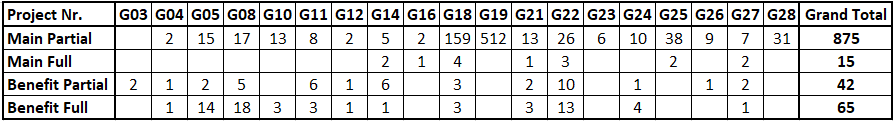
\includegraphics[scale=0.6]{Table/ground_truth.png}
	\captionof{table}{Detail about full and partial redundancies related to main or benefit parts as ground truth}\label{tb:ground_truth}
	
	\endgroup
\end{figure}
As we can see, the main parts of the US-pairs have less full redundancy (15 cases), which means that there are 15 cases where the main part of the US-pairs is exactly the same. This level of redundancy indicates common functionality of the US-pairs, which is a sign of overlapping features. 

A much higher occurrence of partial redundancy in the main parts(875 cases) indicates that there are common elements between the US-pairs, but still enough differences to avoid a complete match. 

Fewer instances of partial redundancy in the benefit parts (42 cases) indicate that the USs diverge in their benefit clauses, they are more tailored to specific project outcomes. 

The higher count of full redundancies (42 cases) compared to partial redundancies in the benefit parts is interesting, as it indicates that the expected objectives of certain features are often repeated in the USs. This suggests that the project is aiming for a set of common goals regardless of the specific functionality.
\subsubsection*{Evaluation of US Redundancy using Tool}
The automated tool is designed to identify redundancy among USs based on predefined criteria. It operates by analysing the text and structure of USs to detect similarities that could indicate redundancy.

In contrast to ground truth, which is based on one-to-one comparison of phrases in specific parts of USs, tool evaluation relies heavily on specified labelling (targets, triggers, contains) using the Doccano tool.

The following criteria are defined for the evaluation of US-pairs:
\begin{itemize}
	\item Full redundancy: 	A pair of US is considered to have "full redundancy" in the main or benefit part when every labelled clause in that part—comprising triggers (in the main part), targets, and contains—is syntactically identical.
	
	\item Partial redundancy: When only some labelled clauses, such as targets, have significant overlap but are not completely identical. This means that while certain labelled clauses, such as targets, may match between USs, other labelled clauses, such as triggers or contains, may differ, meaning that the USs are not fully redundant. This scenario suggests that while USs have significant similarities, they still contain unique aspects.
\end{itemize}
Table \ref{tb:tool} shows the aggregation of the full and partial redundancies in the main and benefit parts assessed by the tool. It is also worth noting that the numbers highlighted in red show the variation in the ground truth evaluation.
\begin{figure}[h]
	\begingroup
	\scriptsize
	\centering
	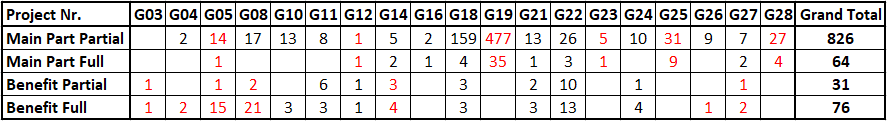
\includegraphics[scale=0.6]{Table/tool.png}
	\captionof{table}{Aggregation of the count of full and partial redundancies in relation to the main or benefit parts assessed by the tool}\label{tb:tool}
	\endgroup
\end{figure}
\paragraph{Assessment of Result: High-Level Overview}Based on the datasets provided, it was found that 1,851 redundancy clauses were identified across all projects, with the highest count found in the backlog G19 dataset (925 clauses), indicating a significant presence of redundancy in the USs of this project. 

Table \ref{tb:redundancy_clauses} shows the total number of redundancy clauses found in each dataset.
\begin{figure}[h]
	\begingroup
	\scriptsize
	\centering
	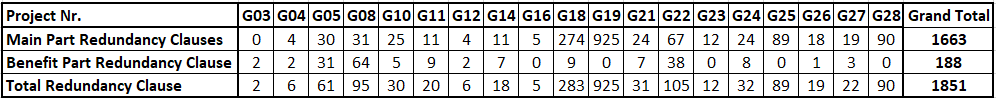
\includegraphics[scale=0.55]{Table/redundancy_clauses.png}
	\captionof{table}{Detail about number of redundancy clauses occurred in main and benefit parts}\label{tb:redundancy_clauses}
	
	\endgroup
\end{figure}
\paragraph{Assessment of Result: Aggregated Analysis}We also look for an aggregate for the count of redundant clauses in both the main and the benefit parts of the USs. 

In the main parts, the large count of full redundancies, especially where two clauses are present (6 clauses), indicates a high degree of similarity in the functionalities described.

In the benefit part of the USs, there is a considerable count of cases where full redundancy prevails, especially where two clauses are inserted (24 clauses). The large count of full redundancies with two clauses indicates that benefits are often described in a standardised way in the different USs.

Figure \ref{fig:aggregation} illustrates the aggregation of the count of redundancy clauses that occur in USs.

\begin{figure}[h]
	\centering
	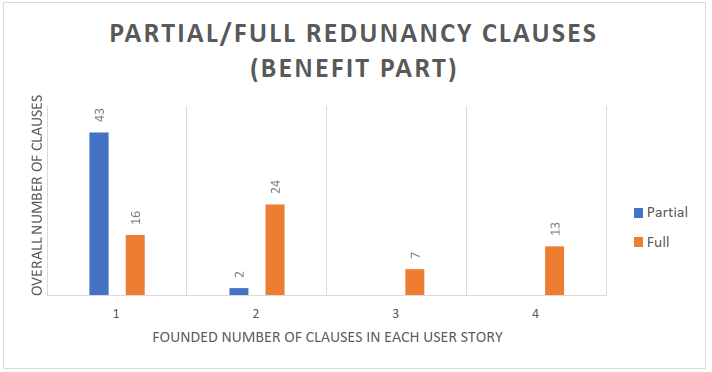
\includegraphics[scale=0.5]{aggregation_benefit}
	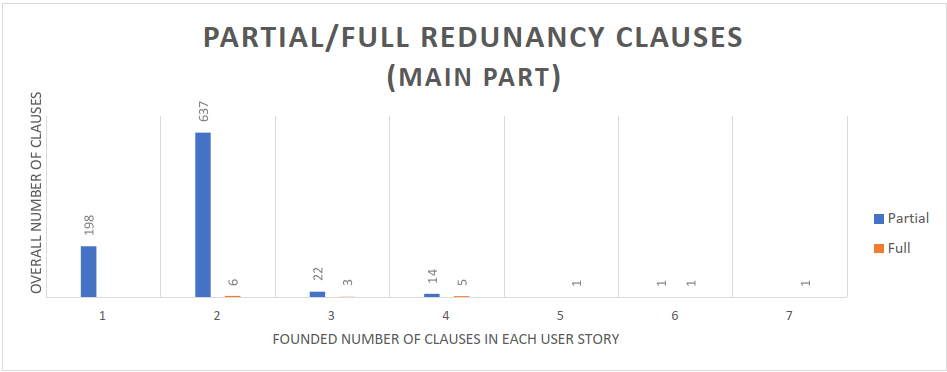
\includegraphics[scale=0.5]{aggregation_main}
	\caption{The aggregation between the count of redundancy clauses occurred in USs}\label{fig:aggregation}
\end{figure}
\paragraph{Assessment of Result: Detailed Insights}In the dataset of Backlog G19, the clause \enquote{have alfred} was repeated in all USs, indicating that \enquote{alfred} is the end product and not a specific functionality. This suggests that the quality of the USs should be considered, so that they do not contain generic information that results in a lot of redundant information(false positives) being provided.

In the main parts of the USs, 1,663 clauses were redundant("Main Part Redundancy Clauses" in Table \ref{tb:redundancy_clauses}), while only 188 redundancy clauses were found in the benefit parts("Benefit Part Redundancy Clauses" in Table \ref{tb:redundancy_clauses}). This means that some USs are not often written in a standardised format for the description of core functions, resulting in a higher count of redundant clauses in the main part.
\begin{example}
	In the dataset of backlog G18 (274 clauses out of 283 in the main parts), for example, this is due to the clauses \enquote{have ability} in the main part, which are unnecessarily repeated in most USs:\\
	\textit{user\_story\_92:} \#g18\# as a \#researcher\# I want to have \#the \#ability\# to search files by file type and format.\\
	\textit{user\_story\_80:} \#g18\# as a \#researcher\# I want to have \#the \#ability\# to attach standard metadata for behavioural observations (and video) so that my data can be searched and understood later.\\
	Actually, the clause \enquote{have ability} in USs should be deleted and no redundancy should be possible at all:\\
	\textit{user\_story\_92:} \#g18\# as a researcher I want to search for files by file type and format.\\
	\textit{user\_story\_80:} \#As a researcher, I want to attach standard metadata for behavioural observations (and videos), so that my data can be searched and understood later.
\end{example}

There are also USs with the same functionality, but one provides more details about the functionality. In other words, one US is contained within another, and we refer to them as full
redundant US-pairs, as deleting the US with less detail has no negative impact on the system. Sometimes it is necessary to merge these two USs to obtain a single detailed US.
\begin{example}
	In the dadaset of backlog G18, for example, we have two US-pairs that are marked as full redundancy between user\_story\_12 and user\_story\_11 as well as user\_story\_13 and user\_story\_11:\\
	\textit{user\_story\_12}: \enquote{\#g18\# as a \#researcher\#, I want to \#upload\# \#files\# prior to having them \#attached\# to a \#log book page\# using the web interface.}\\
	\textit{user\_story\_11:} \enquote{\#g18\# as a \#researcher\#, I want to \#upload\# \#files\# prior to having them \#attached\# to a \#log book page\#.}\\
	\textit{user\_story\_13:} \enquote{\#g18\# as a \#researcher\#, I want to \#upload\# \#files\# prior to having them \#attached\# to a \#log book page\# using a mapped network drive.}\\
	
	As we can see, the user\_story\_11 is an incomplete version of two other USs, and deleting it has no negative impact in the system, due to the fact that its goal is achieved and fulfilled by two other USs.
\end{example}
\paragraph{Research question 1: Conclusion}
After comparing the Ground Truth result with the result provided by our tool, the following realisation was made:
\begin{itemize}
	\item Main Part Partial: A -5.6\% (negative) percentage suggests that the Framework has fewer "Main Part Partial" counts than the Ground Truth.
	In this case, the Framework has about 5.6\% fewer "Main Part Partial" counts than expected.
	
	\item Main Part Full: A high positive percentage of 326.67\% indicates that the Framework has a significantly higher count of Main Part Full compared to Ground Truth.
	At 326.67\%, the framework has more than three times as many main part full compared to the ground truth.
	In our investigation, we found that some phrases are not included as relationship (contains or targets) in the USs annotated with the Doccano tool. Therefore, our tool categorised some USs as fully redundant when in reality they were only partially redundant.
	
	\item Count of Benefit Partial: -26.19\% a negative percentage here indicates that the Framework has fewer "Benefit Partial" counts compared to the Ground Truth.
	With -26.19\%, the Framework has approximately one-quarter fewer "Benefit Partial" counts.
	
	\item Count of Benefit Full: 16.92\% a positive percentage indicates that the Framework has more "Benefit Full" counts compared to the Ground Truth.
	With 16.92\%, the Framework has almost 17\% more "Benefit Full" counts than the Ground Truth.
\end{itemize}
It is also notable that if we add founded partial and full redundancies in main or benefit parts, we both amount are identical(main part: 890 cases , benefit part: 107).

This consistency indicates that the automated tool's results align with the ground truth, suggesting that the tool is reliable in detecting redundancy. It demonstrates that the tool's performance closely matches the personal assessment, reinforcing confidence in its accuracy and validity.
\subsubsection*{Performance Evaluation}
To answer the second research question "How does the tool's performance scale as the count of USs in a backlog increases?", we conducted a series of tests to measure the time it takes the tool to process different counts of USs. This section describes the testing methodology, the results obtained and the impact on the scalability of the tool.
\paragraph{Test Methodology}To evaluate the tool's performance, we conducted a set of experiments in which the tool processed different numbers of USs in a backlog. The tests involved the following steps:
\begin{enumerate}
	\item Backlog Setup: We used backlogs with varying numbers of USs around—50, 70, 90, 120 and 140—to simulate different workload sizes. Each backlog contained USs with varying content, redundancy elements, and complexity to represent a realistic range of cases. Table \ref{tb:performance_env} shows information on the backlog data records provided for the performance test application.
	\begin{figure}[h]
		\begingroup
		\scriptsize
		\centering
		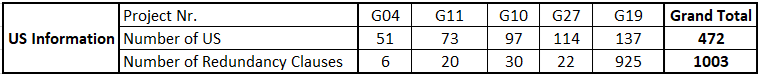
\includegraphics[scale=0.7]{Table/performance_env.png}
		\captionof{table}{Information on the backlog datasets provided for the application of the performance test}\label{tb:performance_env}
		\endgroup
	\end{figure}
	\item Tool Execution: Each part of toolchain(Rule creation, CDA tool, report creation and evaluation) was run for each backlog and the total time taken to process the entire backlog was recorded. The performance of the tool was measured by the processing time, i.e. the total time taken to process all USs in the backlog and identify redundancies.
	
	\item Repeating Tests: To ensure reliability, each test was conducted multiple times, and the average processing time was calculated.
\end{enumerate}
The test environment consisted of:
\begin{itemize}
	\item Processor: Intel(R) Core(TM) i7-8565U CPU @ 1.80GHz (8 CPUs), ~2.0GHz		
	\item Memory: 8070MB RAM
	\item Display Devices: Intel(R) UHD Graphics 620, 4163 MB(Display Memory)
	\item Hard Disk: INTEL SSDPEKNW512G8H
	\item Operating System: Windows 11 Home 64-bit (10.0, Build 22631) (22621.ni\_release.220506-1250)
	\item System Type: 64-bit operating system, x64-based processor
\end{itemize}
Table \ref{tb:performance_result} shows the result of tool's performance in seconds which were conducted on a controlled environment to ensure consistency.

	\begin{figure}[h]
	\begingroup
	\scriptsize
	\centering
	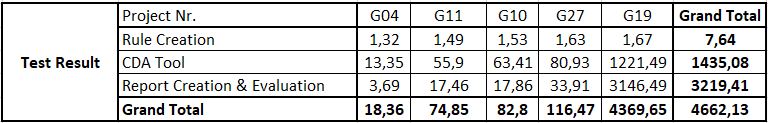
\includegraphics[scale=0.7]{Table/performance_result.png}
	\captionof{table}{Information about the result of the tool's performance test, which was measured using the processing time in seconds.}\label{tb:performance_result}
	\endgroup
\end{figure}
\paragraph{Research question 2: Conclusion}As we can see, there is a direct correlation between the number of USs in a backlog and the time our tool needs to process them. The results confirm that developers and project managers should expect a longer processing time when evaluating redundancy as the backlog grows.

However, the impact on processing time varies depending on the process in question. While rule creation using the Henshin API shows relatively consistent and lower processing times, other components such as the CDA tool and report creation processes show an exponential increase in processing time as the number of USs increases. This indicates that certain processes scale differently as the data load increases.

An important observation is that with a larger number of USs, the probability of finding redundant clauses between USs increases. This has a significant impact on redundancy detection and backlog management specially during processing of CDA tool. As the data set grows, there are more opportunities for overlaps, repetitions or similar USs that could indicate redundancy.
\subsubsection*{Threats to Validity}
When assessing the redundancy of USs through both personal assessment (ground truth) and the automated tool, several potential threats to validity must be considered. This section outlines the main threats to validity and describes how they were mitigated during the study.
\paragraph{Construct validity}It refers to the extent to which the assessment measures what it is intended to measure. The following risks were identified:
\begin{itemize}
	\item Ambiguity of criteria: If the criteria for redundancy are unclear or open to interpretation, this can lead to inconsistent scores. To avoid this, we defined clear and detailed criteria for identifying redundancy in USs.
	
	\item Subjectivity in ground truth: As ground truth is based on personal judgement, subjectivity could lead to bias. To minimise this risk, we cross-checked out evaluations with another experienced evaluator.
\end{itemize}
\paragraph{External validity}External validity refers to the generalisability of the study results to other contexts or population groups. Threats to external validity include:

\begin{itemize}
	\item specificity of USs: If the USs used in the study are too specific or context-dependent, the results may not be transferable to other projects. To mitigate this, we included 19 backlog datasets with different USs and different project types in the analysis.
	
	\item Tool Limitation: The automated tool is designed for a specific format of USs, which limits its broader applicability. Our tool depends heavily on the specific US's format (e.g. "As a \textless user\textgreater, I want to ..., so that..."), which is essential for the application of the tool. Therefore, we tested the tool in isolated contexts limited to well-formed USs and analysed its performance in a number of scenarios.
	
	Another limitation is that our tool is dependent on the specific type of annotation used for USs. In our case, these are annotations such as action, entity, their reference targets, triggers and contains. This means that the effectiveness of the tool depends on the accuracy and consistency of these annotations. If the annotations are incomplete or incorrect, the tool may not work as expected. In addition, the tool may not be compatible with other annotation schemes that do not use these specific labels.
\end{itemize}
\paragraph{Internal Validity}Internal validity is concerned with whether the observed results are attributable to the factors analysed or are influenced by other variables. Potential threats to internal validity include:
\begin{itemize}
	\item Confounding factors: External influences or unintended variables could influence the assessment of redundancy. In particular, USs annotated with Doccano are a very critical impact when evaluating full and partial redundancies between USs using tool. The more phrases are covered in the relationship(targets, contains), the better the score. Since our tool uses Doccano annotated USs as primary input without any changes, these discrepancies are unavoidable. % To avoid this, I controlled the scope of the study to ensure that all user reports came from a consistent context and that consistent evaluation methods were used.
	
	\item Limitation of tool: The automated tool may not capture all aspects of redundancy, especially semantically. This leads us to the next step, the semantic analysis of USs.
\end{itemize}
\subsection{Conclusion}\label{redundancy_conclustion}
In this study, we developed and applied a comprehensive approach that combines the Doccano tool, Henshin and the CDA tool to systematically identify and report redundancies in USs within software development projects with an evaluation.

By carefully analysing 19 different backlog datasets, our method not only separated USs into main and benefit parts for nuanced examination, but also facilitated the distinction between full and partial redundancies within these parts.

Our results reveal a crucial finding: the effectiveness of redundancy detection is significantly influenced by the quality of the USs as well as annotated USs. Well-formulated USs that do not contain unnecessary clauses (e.g. the repetition of \enquote{end product} in all USs) and a concisely annotated backlog specially in relation properties also have a major influence on the effective redundancy analysis process.

 If the main part is evaluated to be full redundant, then we have a US-pair that is functionally identical and we can merge the US-pair into one US. In the case of full redundancy in the benefit part, this means that the US-pairs belong to the same goal and objective, to which they should be categorised for better accessibility and understanding.
 
A notable trend emerged from our analysis: the benefit parts are more often fully redundant than the main parts of USs. This indicates that multiple USs often strive for different functions that contribute to a common system aspect or goal.

Recognising such redundancies not only helps to consolidate functionally identical US-pairs into single, more compact USs, but also to group US-pairs together, improving accessibility and understanding of project backlogs.

In summary, our study confirms the central role of a syntactic analysis approach in detecting and managing redundancies in project backlogs, thereby contributing to the rationalisation of software development processes.

While the quality of annotated USs plays a critical role in the success of this approach, the insights gained from this research provide valuable guidance for both current practices and future research in software project management.

However, our investigation has also shown that we can only consider USs with syntactic redundancy. If they are indeed US-pairs with the same functionality but using different words and clauses to achieve the same goal, we cannot detect this with this approach.

This finding shows that the distinction between actual redundancy and mere superficial similarity can be further refined, which leads us to analyse the USs semantically.

In the next section, we therefore present a method for analysing conflicts and dependencies between USs in semantic way.
%We also find that there are more full redundancy in the benefit part as compared to main part, as the USs with the same benefit achieve different functions for the same aspect of system.

%We have realised that some user stories are only apparently part of other USs, so we can merge them into a compact single US.
%\input{Section/Redundancy_Evaluation}



